\documentclass[12pt,a4paper,final]{article}
\usepackage[utf8]{inputenc}
\usepackage{amsmath}
\usepackage{float}
\usepackage{amsfonts}
\usepackage{amssymb}
\usepackage{graphicx}
\usepackage[margin=1in]{geometry}  
\usepackage{caption}
\usepackage{subcaption}
\begin{document}

\section*{Lab 3 Report}

\subsection*{Part 1 - Camera Calibration}
Calibrate both the left and the right cameras individually. 



Intrinsic parameters, left:
\begin{equation}
\begin{bmatrix}
1702.05& 0 &378.815\\ 0 &1702.81 &245.804 \\0& 0 &1
\end{bmatrix}
\end{equation}
Distortion parameters, left: 
\begin{equation}
\begin{bmatrix}
-0.505677 \\-0.64899 \\-0.000701939 \\-0.0026626 \\13.6816
\end{bmatrix}
\end{equation}

Intrinsic parameters, right:
\begin{equation}
\begin{bmatrix}
1695.75 &0 &357.021 \\0 &1700.72& 255.526 \\0 &0 &1
\end{bmatrix}
\end{equation}
Distortion parameters, right: 
\begin{equation}
\begin{bmatrix}
-0.576054 \\3.30293 \\0.00112569 \\-0.00630633 \\-65.1766
\end{bmatrix}
\end{equation}

%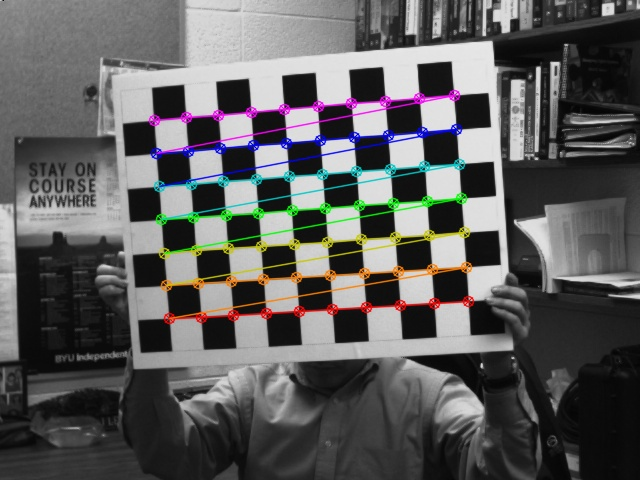
\includegraphics[scale=0.25]{Task_1}

\subsection*{Part 2 - Stereo Calibration}
Rotation Matrix R
\begin{equation*}
\begin{bmatrix}
0.997113 &-0.0139238 &0.0746502 \\0.0142112 &0.999894 &-0.00331927 \\-0.074596 &0.00437056 &0.997204
\end{bmatrix}
\end{equation*}
Translation Matrix T
\begin{equation*}
\begin{bmatrix}
19.6774 & 0.1021 & 0.1679
\end{bmatrix}
\end{equation*}
Essential Matrix E
\begin{equation*}
\begin{bmatrix}
-0.0100026& -0.167419 &0.102379 \\-1.30046 &0.0836638 &19.635 \\-0.381451 &-19.6739 &0.0576925
\end{bmatrix}
\end{equation*}
Fundamental Matrix F
\begin{equation*}
\begin{bmatrix}
-0.0100026 &-0.167419 &0.102379 \\-1.30046 &0.0836638 &19.635 \\-0.381451 &-19.6739 0.0576925
\end{bmatrix}
\end{equation*}

\subsection*{Part 3 - Epipolar Lines}
Compute epipolar lines and show that they pass through the same points on corresponding images.

\begin{figure}[H]
\centering
\begin{subfigure}{.5\textwidth}
  \centering
  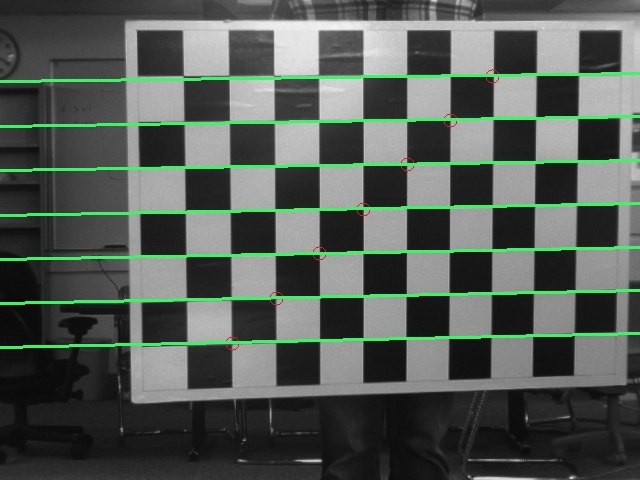
\includegraphics[width=.9\linewidth]{leftEpi}
  \caption{Left camera with epipolar lines}
  \label{fig:sub1}
\end{subfigure}%
\begin{subfigure}{.5\textwidth}
  \centering
  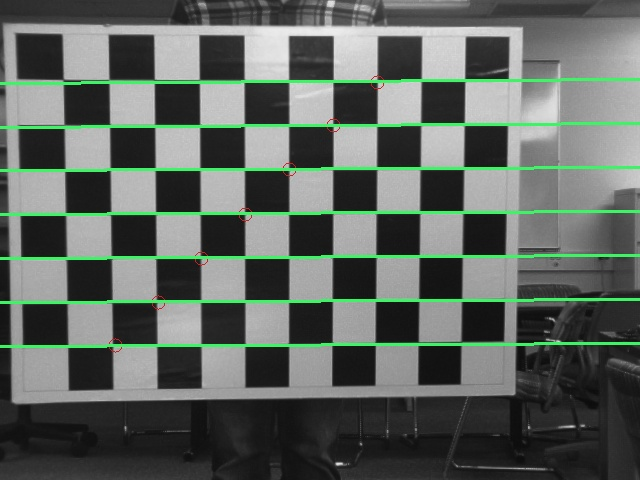
\includegraphics[width=.9\linewidth]{rightEpi}
  \caption{Right camera with epipolar lines}
  \label{fig:sub2}
\end{subfigure}
\label{fig:test}
\end{figure}

\subsection*{Part 4 - Rectification}

Rectify the left and right stereo image and show that points line up horizontally on both images.

\begin{figure}[H]
\centering
\begin{subfigure}{.5\textwidth}
  \centering
  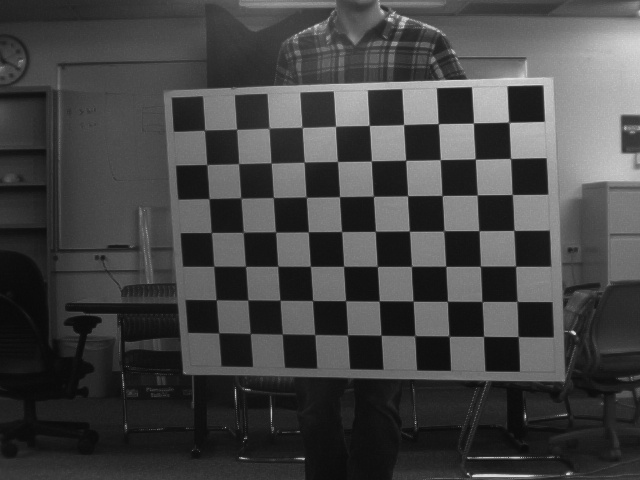
\includegraphics[width=.9\linewidth]{origRemapL}
  \caption{Original Left}
  \label{fig:sub1}
\end{subfigure}%
\begin{subfigure}{.5\textwidth}
  \centering
  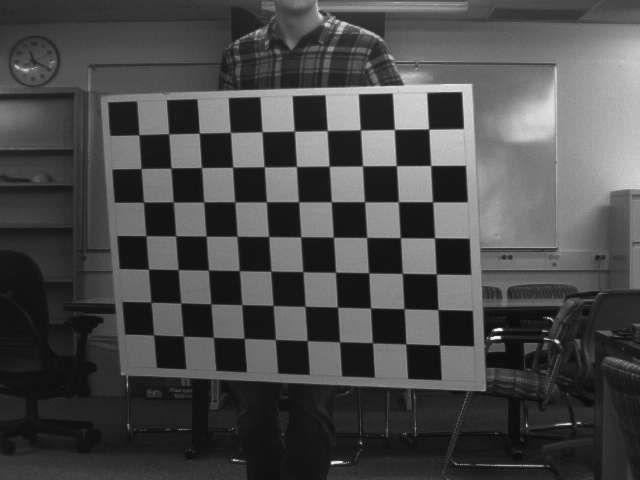
\includegraphics[width=.9\linewidth]{origRemapR}
  \caption{Original Right}
  \label{fig:sub2}
\end{subfigure}
\label{fig:test}
\end{figure}


\begin{figure}[H]
\centering
\begin{subfigure}{.5\textwidth}
  \centering
  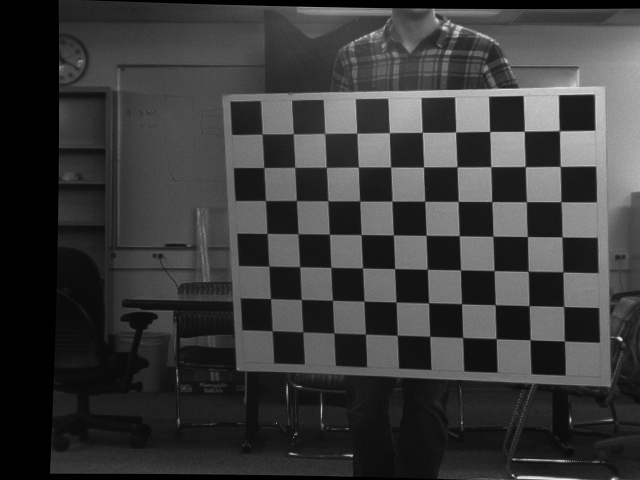
\includegraphics[width=.9\linewidth]{RemapL}
  \caption{Rectified Left}
  \label{fig:sub1}
\end{subfigure}%
\begin{subfigure}{.5\textwidth}
  \centering
  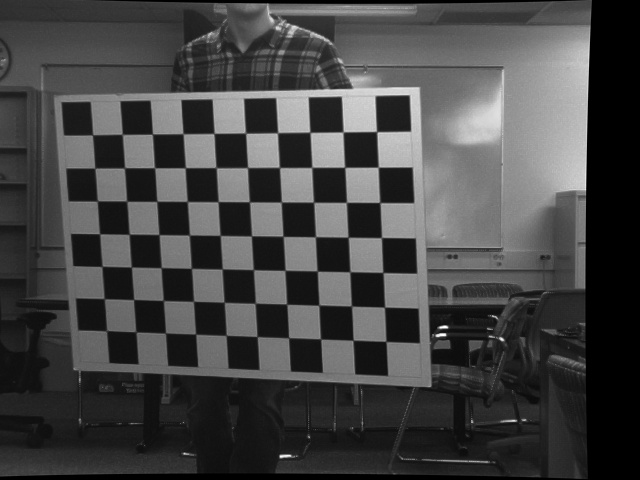
\includegraphics[width=.9\linewidth]{RemapR}
  \caption{Rectified Right}
  \label{fig:sub2}
\end{subfigure}
\label{fig:test}
\end{figure}

\begin{figure}[H]
\centering
\begin{subfigure}{.5\textwidth}
  \centering
  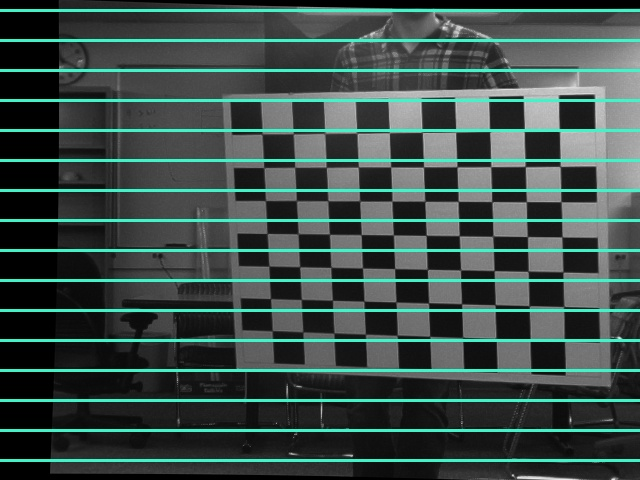
\includegraphics[width=.9\linewidth]{linesRemapL}
  \caption{Lines through rectified left}
  \label{fig:sub1}
\end{subfigure}%
\begin{subfigure}{.5\textwidth}
  \centering
  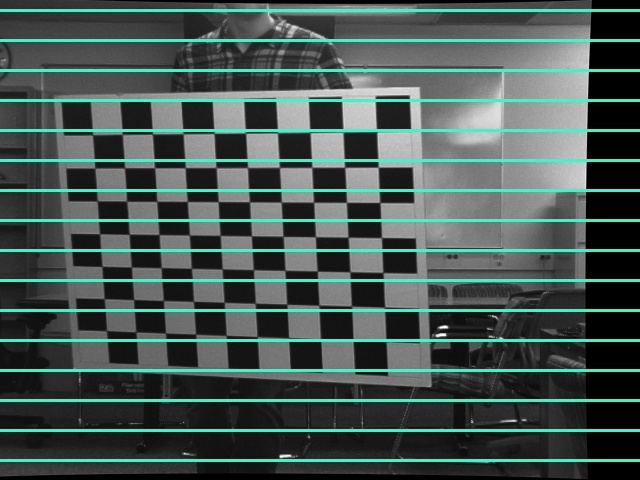
\includegraphics[width=.9\linewidth]{linesRemapR}
  \caption{Lines through rectified right}
  \label{fig:sub2}
\end{subfigure}
\label{fig:test}
\end{figure}


\begin{figure}[H]
\centering
\begin{subfigure}{.5\textwidth}
  \centering
  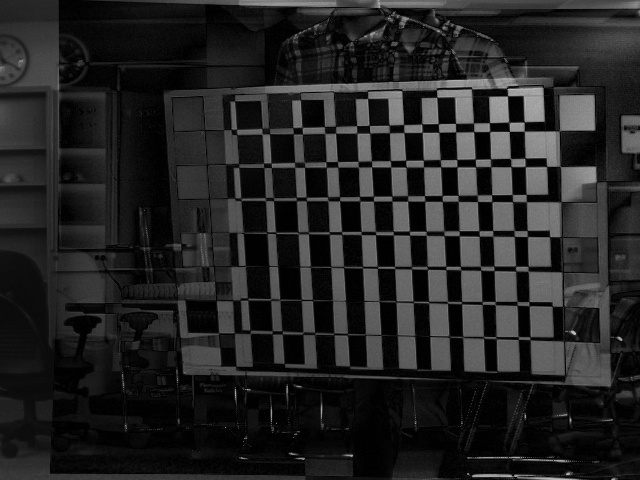
\includegraphics[width=.9\linewidth]{remapDiffL}
  \caption{Left Diff}
  \label{fig:sub1}
\end{subfigure}%
\begin{subfigure}{.5\textwidth}
  \centering
  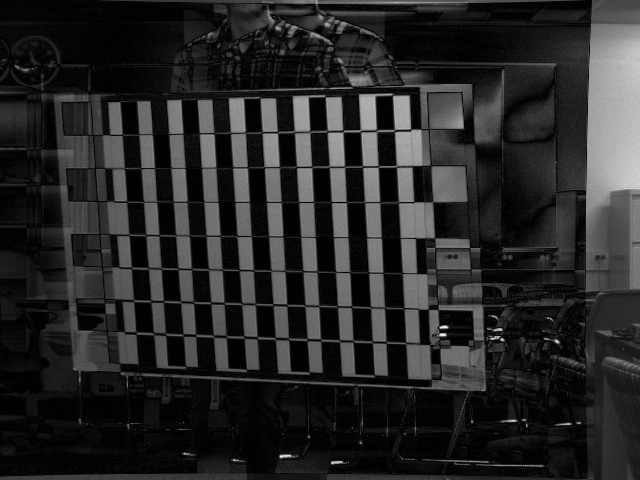
\includegraphics[width=.9\linewidth]{remapDiffR}
  \caption{Right Diff}
  \label{fig:sub2}
\end{subfigure}
\label{fig:test}
\end{figure}



\subsection*{Part 5 - 3D Measurement}
Measure the distance between known 3D points (chessboard corners) and verify accuracy.

\begin{figure}[H]
\centering
\begin{subfigure}{.5\textwidth}
  \centering
  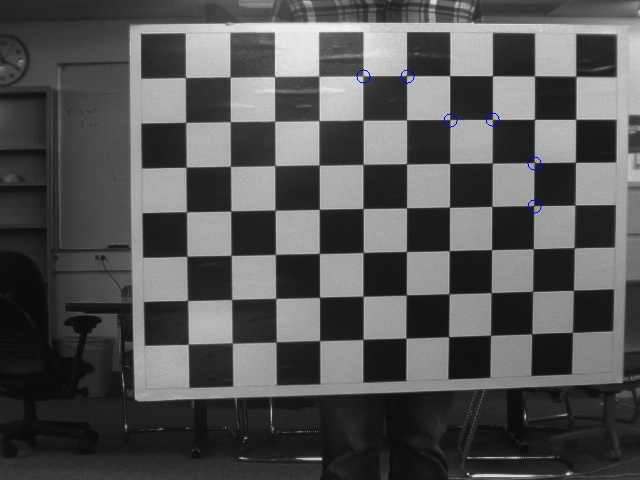
\includegraphics[width=.9\linewidth]{measurementL}
  \caption{Left measurement points}
  \label{fig:sub1}
\end{subfigure}%
\begin{subfigure}{.5\textwidth}
  \centering
  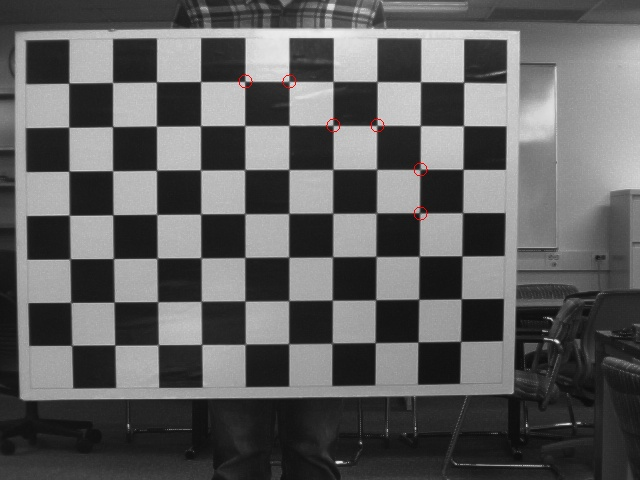
\includegraphics[width=.9\linewidth]{measurementR}
  \caption{Right measurement points}
  \label{fig:sub2}
\end{subfigure}
\label{fig:test}
\end{figure}

I measured the distance between points. Starting with the top left point, I measured the distance to one square over (3.8827 inches), to one square diagonally down (5.4921 inches), to one square over (3.8870 inches), to one square diagonally down(5.4944 inches), to one square down (3.8706 inches). I did this by taking a three-dimensional distance between points with respect to the same camera, i.e. from point $\{x_i, y_i, z_i\}_{left}$ to $\{x_i, y_i, z_i\}_{right}$. Since I selected the points using the findChessboardCorners function, I can expect them to be almost exactly on the corners, leading to the highly accurate (2 decimal places) calculation of 3-dimensional distance. (5.49 is about equal to the $\sqrt{3.88^2 + 3.88^2}$).

\end{document}